\only<beamer>{\titleframe}

\begin{frame}{Gliederung}
  \tableofcontents
\end{frame}


\section{Einführung}
\begin{frame}{\insertsection}
  \textit{Selection:} Select the $i$-th smallest element in a list with $n$ elements.

  \vspace{5mm}
  Previous works:

  \vspace{5mm}
  \begin{tabular}{|p{5cm}|p{5cm}|}
    \hline
    Gasarch, Kelly, and Puth                                               & Oksanen   \\
    \hline
    \raggedright \begin{itemize}
                   \item Introduced computer search to find optimal selection algorithms.
                   \item ...
                 \end{itemize} &
    \raggedright \begin{itemize}
                   \item Published a computer search algorithm improving the previously known lower bounds found
                         by Gasarch et. al.
                 \end{itemize}
  \end{tabular}
\end{frame}


\section{Grundlagen}
\sectionframe{\insertsection}
\begin{frame}{\insertsection}
  $$ \Omega = \{ a,b,c,...\}, \quad |\Omega| = n $$
  $$P = (n,i,R), \quad R \subseteq \Omega^2$$
\end{frame}

\begin{frame}{\insertsection}
  \centering
  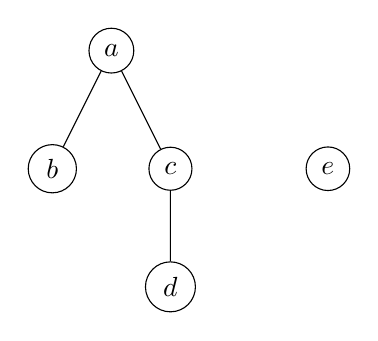
\begin{tikzpicture}

    \node[draw, circle] (a) {$a$}
    child {
        node[draw, circle] {$b$}
      }
    child {
        node[draw, circle] (c) {$c$}
        child {
            node[draw, circle] {$d$}
          }
      }
    ;

    \node[draw, circle, right of=c, node distance=2cm] {$e$};

  \end{tikzpicture}

  \begin{align*}
    a & > b \\
    a & > c \\
    c & > d
  \end{align*}
\end{frame}

\subsection{Kompatiblen Lösungen}
\begin{frame}{\insertsubsection}
  \centering
  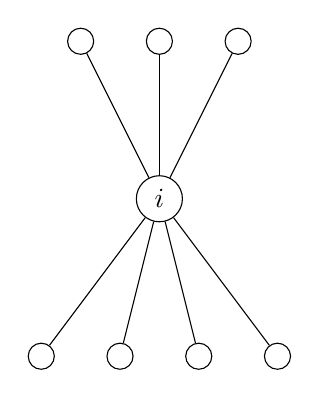
\begin{tikzpicture}

    \node[draw, circle] (l0) at (0, 0) {};
    \node[draw, circle] (l1) at (1, 0) {};
    \node[draw, circle] (l2) at (2, 0) {};
    \node[draw, circle] (l3) at (3, 0) {};

    \node[draw, circle] (I) at (1.5, 2) {$i$};

    \path[draw] (l0) to (I);
    \path[draw] (l1) to (I);
    \path[draw] (l2) to (I);
    \path[draw] (l3) to (I);

    \node[draw, circle] (u0) at (0.5, 4) {};
    \node[draw, circle] (u1) at (1.5, 4) {};
    \node[draw, circle] (u2) at (2.5, 4) {};

    \path[draw] (u0) to (I);
    \path[draw] (u1) to (I);
    \path[draw] (u2) to (I);

  \end{tikzpicture}

\end{frame}

\begin{frame}{\insertsubsection}
  \centering
  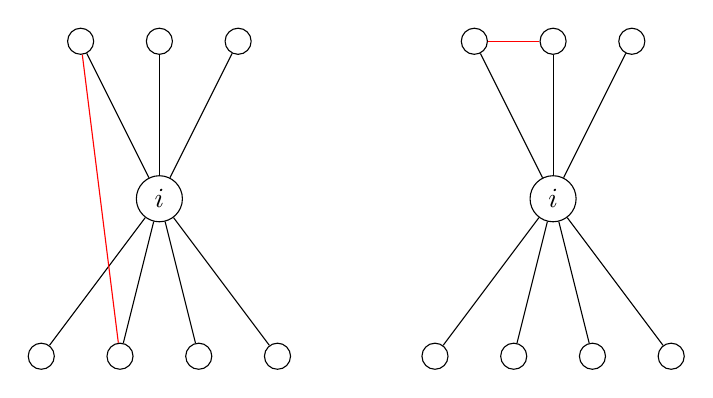
\begin{tikzpicture}

    \node[draw, circle] (fl0) at (0, 0) {};
    \node[draw, circle] (fl1) at (1, 0) {};
    \node[draw, circle] (fl2) at (2, 0) {};
    \node[draw, circle] (fl3) at (3, 0) {};

    \node[draw, circle] (fI) at (1.5, 2) {$i$};

    \path[draw] (fl0) to (fI);
    \path[draw] (fl1) to (fI);
    \path[draw] (fl2) to (fI);
    \path[draw] (fl3) to (fI);

    \node[draw, circle] (fu0) at (0.5, 4) {};
    \node[draw, circle] (fu1) at (1.5, 4) {};
    \node[draw, circle] (fu2) at (2.5, 4) {};

    \path[draw] (fu0) to (fI);
    \path[draw] (fu1) to (fI);
    \path[draw] (fu2) to (fI);

    \path[draw=red] (fu0) to (fl1);

    %second

    \node[draw, circle] (sl0) at (0 + 5, 0) {};
    \node[draw, circle] (sl1) at (1 + 5, 0) {};
    \node[draw, circle] (sl2) at (2 + 5, 0) {};
    \node[draw, circle] (sl3) at (3 + 5, 0) {};

    \node[draw, circle] (sI) at (1.5 + 5, 2) {$i$};

    \path[draw] (sl0) to (sI);
    \path[draw] (sl1) to (sI);
    \path[draw] (sl2) to (sI);
    \path[draw] (sl3) to (sI);

    \node[draw, circle] (su0) at (0.5 + 5, 4) {};
    \node[draw, circle] (su1) at (1.5 + 5, 4) {};
    \node[draw, circle] (su2) at (2.5 + 5, 4) {};

    \path[draw] (su0) to (sI);
    \path[draw] (su1) to (sI);
    \path[draw] (su2) to (sI);

    \path[draw=red] (su0) to (su1);

  \end{tikzpicture}

\end{frame}


\section{Vorwärtssuche}
\sectionframe{\insertsection}
\begin{frame}{\insertsection}

\end{frame}

\begin{frame}{\insertsection}
  \centering
  \begin{tikzpicture}
    [
      level 1/.style = {sibling distance = 4cm},
      level 2/.style = {sibling distance = 2.5cm},
    ]

    \node[] (root) {$(n,i,\emptyset)$}
    child {
        node[] {$\{a,b\}$}
        child {
            node[] {$(n,i,\{(a,b)\})$}
            child[sibling distance = 1cm] {
                node[] {$\{c,d\}$}
                child[sibling distance = 1cm] { node[] {$\cdots$}}
                child[sibling distance = 1cm] { node[] {$\cdots$}}
              }
            child[sibling distance = 1cm] { node[] {$\cdots$}}
          }
        child {
            node[] {$(n,i,\{(b,a)\})$}
            child[sibling distance = 1cm] {
                node[] {$\{c,d\}$}
                child[sibling distance = 1cm] { node[] {$\cdots$}}
                child[sibling distance = 1cm] { node[] {$\cdots$}}
              }
            child[sibling distance = 1cm] { node[] {$\cdots$}}
          }
      }
    child {
        node {$\{a,c\}$}
        child[sibling distance = 1cm] { node[] {$\cdots$}}
        child[sibling distance = 1cm] { node[] {$\cdots$}}
      }
    child {
        node[] {$\cdots$}
      }
    ;

  \end{tikzpicture}

\end{frame}

\subsection{Multithreading}
\begin{frame}{\insertsubsection}

\end{frame}


\section{Rückwärtssuche}
\sectionframe{\insertsection}
\begin{frame}{\insertsection}
  % - backward search starts with the solved poset
  % - iteratively removes comparisons until the searched poset is found

  % $P_{\text{unordered} (1, 0)} = (1, 0, \emptyset)$

  % ...
\end{frame}

\begin{frame}{\insertsection}
  % Idee: interaktiv an Tafel
  % Ebene k enthält alle Posets, die in k Vergleichen gelöst werden können und durch vorherigen Ebene(n) gebildet werden können
  % ganze Pfeile: zeigen auf Poset in Ebene k - 1, das durch Entfernen eines Vergleichs resultiert
  % gestrichelte Pfeile: zeigen auf Poset, das resultiert Umkehrvergleich eingefügt wird (alle Ebenen kleiner k)
  % Rückwärtssuche startet unten bei k = 0, einzigem "gelösten" Poset
  % berechne Ebene k + 1 wie folgt:
  %  - versuche zunächst einen Vergleich zu entfernen
  %  - füge Element mit Vergleichen hinzu, sodass lösbarkeit nicht beeinfluss & entferne anschließend Vergleich
  %  - 

  \begin{figure}[!b]
    \centering
    \includegraphics[width=0.9\textwidth,height=0.67\textheight,keepaspectratio]{./figures/backward-searchtree-bound3.png}
    \caption{$n=4,i=1,\text{obere Schranke}=3$}
    \label{fig:backward-searchtree-bound3}
  \end{figure}
\end{frame}

\begin{frame}{\insertsection}
  \begin{figure}[!b]
    \centering
    \includegraphics[width=0.9\textwidth,height=0.67\textheight,keepaspectratio]{./figures/backward-searchtree-bound4.png}
    \caption{$n=4,i=1,\text{obere Schranke}=4$}
    \label{fig:backward-searchtree-bound4}
  \end{figure}

\end{frame}

\begin{frame}{\insertsection~--~Multithreading}
  % 1  core : 7h 2m 59s
  % 32 cores:   20m 11s

  \begin{figure}
    \centering
    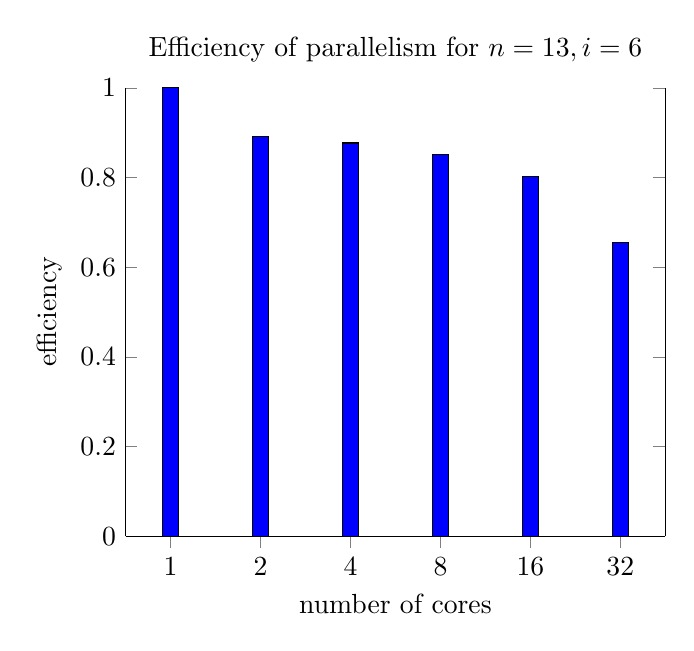
\begin{tikzpicture}
      \begin{axis}[
          ymin=0,
          ymax=1,
          axis x line=bottom,
          enlarge x limits=0.1,
          x axis line style={-},
          ylabel={efficiency},
          xlabel={number of cores},
          title={Efficiency of parallelism for $n = 13, i = 6$},
          ybar, % This makes the plot a bar chart
          bar width=0.2cm, % Adjust bar width
          % nodes near coords, % Display values on top of bars
          xtick=data, % Set x-ticks to data points
          symbolic x coords={1, 2, 4, 8, 16, 32}, % Specify the x-tick labels
        ]
        \addplot[
          ybar,
          fill=blue
        ] coordinates {
            (1, 1.000)
            (2, 0.892)
            (4, 0.877)
            (8, 0.851)
            (16, 0.803)
            (32, 0.655)
          };
      \end{axis}
    \end{tikzpicture}
  \end{figure}

  $\text{efficiency} = (\text{single-core time}) \div (\text{number of cores} \cdot \text{multi-core time})$ \\
\end{frame}

\begin{frame}{\insertsection}
  \begin{figure}[!b]
    \centering
    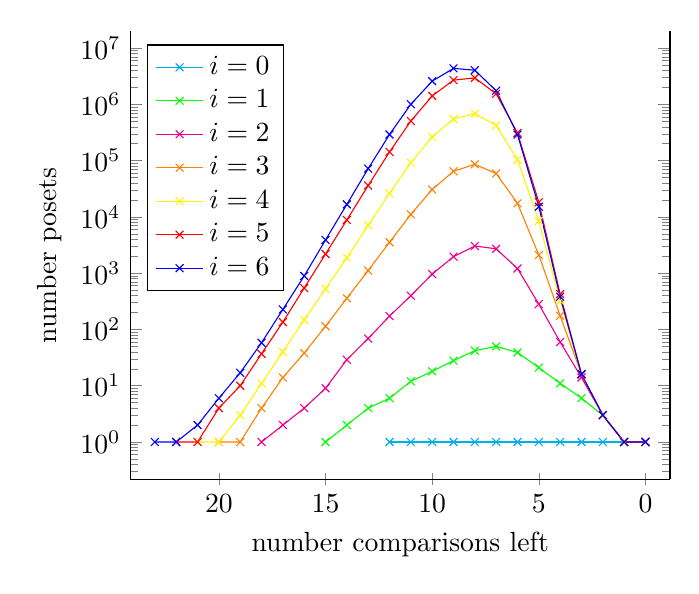
\begin{tikzpicture}
  \begin{axis}[
      ymode=log,
      axis x line = bottom,%x-Achse nur unten
      x dir=reverse,
      enlarge x limits = .05,%x-Achse erweitern
      x axis line style = {-},%kein Pfeil
      % title = {\dots},
      ylabel={number posets},
      xlabel={number comparisons left},
      % only marks,
      cycle list={{mark=x}},
      legend pos=north west,
    ]
    \addlegendentry{$i = 0$}
    \addplot+[cyan] table { %n=13,i=0
        x  y
        0  1
        1  1
        2  1
        3  1
        4  1
        5  1
        6  1
        7  1
        8  1
        9  1
        10 1
        11 1
        12 1
      };
    \addlegendentry{$i = 1$}
    \addplot+[green] table { %n=13,i=1
        x y
        0  1
        1  1
        2  3
        3  6
        4  11
        5  21
        6  39
        7  50
        8  42
        9  28
        10 18
        11 12
        12 6
        13 4
        14 2
        15 1
      };
    \addlegendentry{$i = 2$}
    \addplot+[magenta] table { %n=13,i=2
        x y
        0  1
        1  1
        2  3
        3  14
        4  60
        5  282
        6  1211
        7  2714
        8  3043
        9  1966
        10 964
        11 398
        12 173
        13 69
        14 29
        15 9
        16 4
        17 2
        18 1
      };
    \addlegendentry{$i = 3$}
    \addplot+[orange] table { %n=13,i=3
        x y
        0  1
        1  1
        2  3
        3  16
        4  175
        5  2110
        6  17421
        7  59192
        8  86141
        9  64764
        10 30751
        11 11099
        12 3551
        13 1115
        14 359
        15 114
        16 38
        17 14
        18 4
        19 1
        20 1
      };
    \addlegendentry{$i = 4$}
    \addplot+[yellow] table { %n=13,i=4
        x y
        0  1
        1  1
        2  3
        3  16
        4  323
        5  8486
        6  104001
        7  422605
        8  685670
        9  550976
        10 265263
        11 91793
        12 26319
        13 7107
        14 1891
        15 526
        16 148
        17 40
        18 11
        19 3
        20 1
        21 1
      };
    \addlegendentry{$i = 5$}
    \addplot+[red] table { %n=13,i=5
        x y
        0  1
        1  1
        2  3
        3  16
        4  425
        5  18246
        6  310677
        7  1545376
        8  2960442
        9  2703528
        10 1414495
        11 506441
        12 143196
        13 36191
        14 8860
        15 2190
        16 545
        17 135
        18 37
        19 10
        20 4
        21 1
        22 1
      };
    \addlegendentry{$i = 6$}
    \addplot+[blue] table { % n=13,i=6
        x y
        0  1
        1  1
        2  3
        3  16
        4  381
        5  15227
        6  290138
        7  1750707
        8  4058631
        9  4368185
        10 2592437
        11 1006071
        12 291970
        13 72346
        14 16728
        15 3898
        16 893
        17 227
        18 58
        19 17
        20 6
        21 2
        22 1
        23 1
      };
  \end{axis}
\end{tikzpicture}
    % \caption{Number of posets generated by the backward search for $n = 14$ depending on the number of comparisons for various $i$. Be aware of the logarithmic scale of the y-axis and that the reverse search does not add comparisons, but rather removes them.}
    % \label{fig:backward-posets-per-level}
  \end{figure}
\end{frame}


\section{Bidirektionale Suche}
\sectionframe{\insertsection}
\begin{frame}{\insertsection}
  Bidirectional search

\end{frame}

\begin{frame}{\insertsection}
  \begin{figure}[!b]
    \centering
    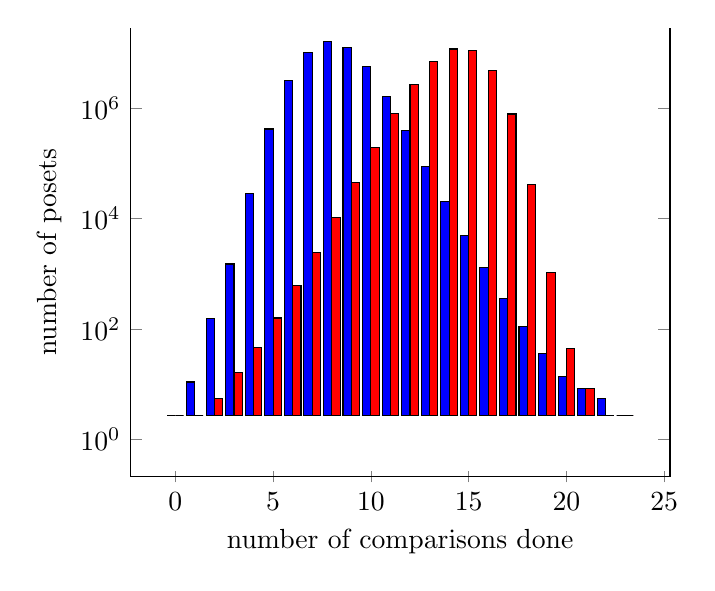
\begin{tikzpicture}
  \begin{axis}[
      ybar,
      ymode=log,
      axis x line = bottom,%x-Achse nur unten
      enlarge x limits = .1,%x-Achse erweitern
      x axis line style = {-},%kein Pfeil
      bar width=3pt,
      ylabel={number of posets},
      xlabel={number of comparisons done},
      % legend cell align=left,
      % legend pos=outer north east,
      % legend style={at={(0.5,-0.2)},anchor=north}, % draw=none
    ]
    % \addlegendentry{forward search}
    \addplot[fill=blue,shift={(1pt, 0)}] table {
        x y
        0  1
        1  4
        2  57
        3  552
        4  10397
        5  154828
        6  1166640
        7  3770182
        8  5941732
        9  4726819
        10 2096404
        11 604582
        12 143058
        13 32460
        14 7450
        15 1823
        16 471
        17 132
        18 41
        19 13
        20 5
        21 3
        22 2
        23 1
      };
    % \addlegendentry{backward search}
    \addplot[fill=red,shift={(-1pt, 0)}] table {
        x y
        23 1
        22 1
        21 3
        20 16
        19 381
        18 15227
        17 290138
        16 1750707
        15 4058631
        14 4368185
        13 2592437
        12 1006071
        11 291970
        10 72346
        9  16728
        8  3898
        7  893
        6  227
        5  58
        4  17
        3  6
        2  2
        1  1
        0  1
      };
  \end{axis}
\end{tikzpicture}
    % \caption{Number of posets depending on the number of comparisons for $n = 13$ and $i = 6$ (red: backward search, blue: forward search).}
    % \label{fig:backward_forward_count_13_6}
  \end{figure}

  {\color{red} Rot: Rückwärtssuche},
  {\color{blue} Blau: Vorwärtssuche}
\end{frame}


\section{Ergebnisse}
\sectionframe{\insertsection}

\begin{frame}{\insertsection}
  % hier kommt fehler von oksanen hin (falsche Heuristik,, führt zu falschem wert)

  % hier kommt faslche these von gasarch
\end{frame}

\begin{frame}{\insertsection}
  \begin{table}[!t]
    \renewcommand{\arraystretch}{0.9}
    \centering
    \resizebox{0.9\textheight}{!}{%
    \begin{tabular}{c|cccccccc}
      \backslashbox{$n$}{$i$} & 0  & 1  & 2  & 3  & 4  & 5  & 6  & 7  \\ \hline
      1                       & 0                                     \\
      2                       & 1                                     \\
      3                       & 2  & 3                                \\
      4                       & 3  & 4                                \\
      5                       & 4  & 6  & 6                           \\
      6                       & 5  & 7  & 8                           \\
      7                       & 6  & 8  & 10 & 10                     \\
      8                       & 7  & 9  & 11 & 12                     \\
      9                       & 8  & 11 & 12 & 14 & 14                \\
      10                      & 9  & 12 & 14 & 15 & 16                \\
      11                      & 10 & 13 & 15 & 17 & 18 & 18           \\
      12                      & 11 & 14 & 17 & 18 & 19 & 20           \\
      13                      & 12 & 15 & 18 & 20 & 21 & 22 & 23      \\
      14                      & 13 & 16 & 19 & 21 & 23 & 24 & 25      \\
      15                      & 14 & 17 & 20 & 23 & 24 & 26 & 26 & 27 \\
    \end{tabular}%
    }
  \end{table}
\end{frame}

\thanksframe

% \begin{frame}{Quellen}
%   \nocite{*}
%   \printbibliography
% \end{frame}